\documentclass[conference]{IEEEtran}
\IEEEoverridecommandlockouts
% The preceding line is only needed to identify funding in the first footnote. If that is unneeded, please comment it out.
\usepackage{cite}
\usepackage{amsmath,amssymb,amsfonts}
\usepackage{algorithmic}
\usepackage{textcomp}
\usepackage{xcolor}
\usepackage{tikz}
\definecolor{titlepagecolor}{cmyk}{.5,.0,.40,.60}

\DeclareFixedFont{\titlefont}{T1}{ppl}{b}{it}{0.5in}

\makeatletter                       
\def\printauthor{%                  
	{\large \@author}}              
\makeatother
\author{%
	Gordan Konevski \\
	\texttt{gordan.konevski@stud.hshl.de} \\
	Hochschule Hamm-Lippstadt, 2021
}


\def\BibTeX{{\rm B\kern-.05em{\sc i\kern-.025em b}\kern-.08em
		T\kern-.1667em\lower.7ex\hbox{E}\kern-.125emX}}
	
\begin{document}

\title{Slack Stealing}
\maketitle

\begin{abstract}
This paper deals with the uses and relevancy of slack stealing in embedded real-time systems. It ultimately aims to define the environment in which it is typically used as a method and, through  some examples, show its use in practice, in order to prove it as a viable and useful method.
\end{abstract}

\section {Real-Time Systems}
\subsection{Basic Concept}
Typically software is seen through the perspective of an interactive system, in which the user issues commands that are (typically) visibly displayed.  Interactive software, as it is referred to, is
always subject to delays. It is this time delay that we wish to distinguish from software that is based on real-time systems. We may define it as such 

\begin{figure}[h!]
	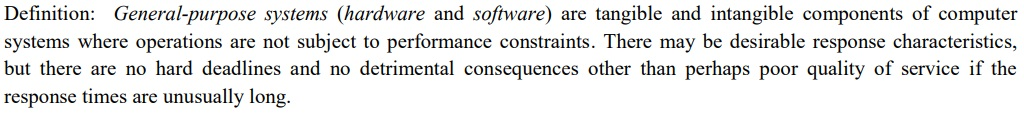
\includegraphics[width=8cm, height=1cm]{def1}
	\caption{General Definition}
	\centering
\end{figure}

In contrast with general-purpose systems, real-time systems are meant to monitor, interact with, control, or respond to the physical environment. The interface is set-up through sensors, communications systems, actuators, and other input and output devices. Under such circumstances, it is necessary to respond to incoming information in a timely manner. Delays may prove dangerous or even catastrophic. Consequently, we will define a real-time system as one where:
\begin{itemize}
	\item the time at which a response is delivered is as important as the correctness of that response. So whether a command is executed within the specified time range is as important as the command itself, and a failure to execute the command on time is regarded as a fatal error.
	\item the consequences of a late response are just as hazardous as the consequences of an incorrect response.
\end{itemize}
Those requirements that describe how the system should respond to a given set of inputs (both from sensors and
messages received from communication systems) given the current state of the system and what the expected outputs
(both signals to actuators and messages sent through communication systems) and changes of state of the system are
described as functional requirements.
Other non-functional requirements may include availability, configurability and regulatory compliance. Real-time
systems are not meant to be fast, per se; instead, they should be just fast enough to ensure that all functional requirements
and non-functional requirements including, but not limited to, performance requirements.
Some examples of real time systems include:
\begin{itemize}
	\item transportation, for e.g. control systems for vehicles, spacecrafts, ships etc.
	\item telecommunication
	\item building management: security, heating, ventilation, air conditioning and lighting
	\item production control in an industrialized environment
\end{itemize}
\begin{figure}[h!]
	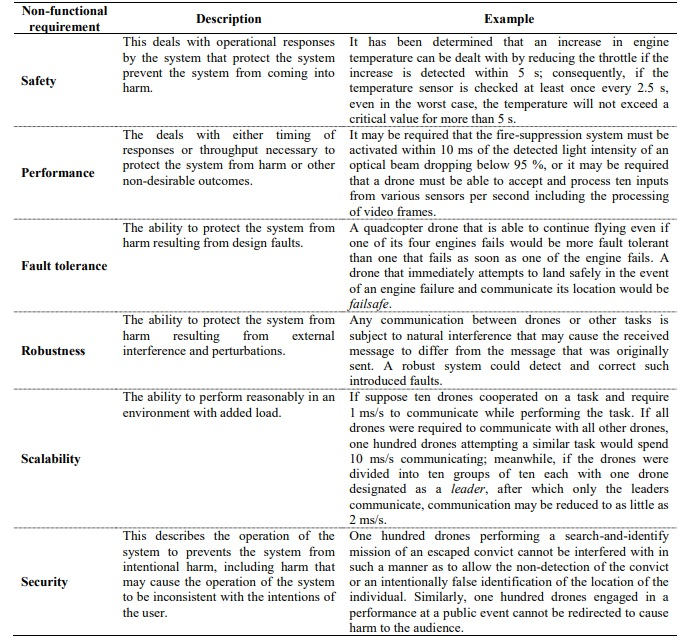
\includegraphics[width=8cm, height=8cm]{table1}
	\caption{Some Non-Functional Requirements of Real-Time Systems}
	\centering
\end{figure}

\subsection{Defining Time}
A highly technical definition of time would be that time is a natural phenomenon where one “second” is the duration of exactly 9192631770 periods of the radiation corresponding to the transition between the two
hyperfine levels of the ground state of the caesium 133 atom at rest at a temperature of 0 Kelvin,
as defined by the Bureau international des poids et mesures. With the exception of the kilogram, all other units are
defined relative to the second. Atomic clocks are used to measure time, and coordinated universal time (UTC) is an
international standard for time. But most systems, however, use quartz clocks, where a quartz crystal is carved to
vibrate at 215 Hz = 32768 Hz when an electric field is placed across it. A 5-bit digital counter will overflow once per
second as it counts the oscillations. With 86400 s/day, such clocks tend to drift less than 1 s/day and therefore different
systems will have different times even if they start synchronized (more expensive crystals will have less drift). Depending on the system in place, the accuracy of the clock vary in their importance. Naturally, systems built for e.g. astrophysical research require atomic clocks as opposed to quartz clocks.

\section {Slack Stealing}

A big portion of the scheduling algorithms used deal with homogeneous
sets of tasks, where all computational activities are either aperiodic or periodic. It may just be the case, however, that certain systems require both types of processes, which may
also differ in their criticality. Typically, periodic tasks are time-driven and execute
critical control activities with hard timing constraints aimed at guaranteeing regular
activation rates. Aperiodic tasks, on the other hand, are usually event-driven and may have hard, soft, or
non-real-time requirements depending on the specific application.
When dealing with hybrid task sets, the main objective of the kernel is to guarantee the
schedulability of all critical tasks in worst-case conditions and provide good average
response times for soft and non-real-time activities. Off-line guarantee of event-driven
aperiodic tasks with critical timing constraints can be done only by making proper
assumptions on the environment; that is, by assuming a maximum arrival rate for
each critical event. This implies that aperiodic tasks associated with critical events are
characterized by a minimum interarrival time between consecutive instances, which
bounds the aperiodic load. Aperiodic tasks characterized by a minimum inter-arrival
time are called sporadic. They are guaranteed under peak-load situations by assuming
their maximum arrival rate.
If the maximum arrival rate of some event cannot be bounded a priori, the associated
aperiodic task cannot be guaranteed off-line, although an online guarantee of individual aperiodic requests can still be done. Aperiodic tasks requiring online guarantee
on individual instances are called firm. Whenever a firm aperiodic request enters the
system, an acceptance test can be executed by the kernel to verify whether the request can be served within its deadline. If such a guarantee cannot be done, the request is
rejected.
In the next sections, we present a number of scheduling algorithms for handling hybrid
task sets consisting of a subset of hard periodic tasks and a subset of soft aperiodic
tasks. All algorithms presented in this chapter rely on the following assumptions:
	\begin{itemize}
	\item Periodic tasks are scheduled based on a fixed-priority assignment; namely, the
	Rate-Monotonic (RM) algorithm;
	\item All periodic tasks start simultaneously at time t = 0 and their relative deadlines
	are equal to their periods.
	\item Arrival times of aperiodic requests are unknown.
	\item When not explicitly specified, the minimum inter-arrival time of a sporadic task is
	assumed to be equal to its deadline.
	\item All tasks are fully preemptable.
	\item Aperiodic scheduling under dynamic priority assignment is discussed in the next chapter.
\end{itemize}

The Slack Stealing algorithm is another aperiodic service technique, which offers substantial improvements in response time over alternative service methods. Unlike such methods, the Slack Stealing algorithm does not create a periodic server for aperiodic task
service. Rather it creates a passive task, referred to as the Slack Stealer, which attempts
to make time for servicing aperiodic tasks by “stealing” all the processing time it can
from the periodic tasks without causing their deadlines to be missed. This is equivalent to stealing slack from the periodic tasks. We recall that if ci(t) is the remaining computation time at time t, the slack of a task Ti is: 

\begin{figure}[h!]
	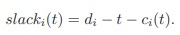
\includegraphics[width=8cm, height=1.5cm]{alg1.jpg}
	\caption{Slack Stealing Task}
	\centering
\end{figure}

The main idea behind slack stealing is that, typically, there is no benefit in early completion of the periodic tasks. Hence, when an aperiodic request arrives, the Slack Stealer steals all the available slack from periodic tasks and uses it to execute aperiodic requests as soon as possible. If no aperiodic requests are pending, periodic tasks
are normally scheduled by Rate Monotonic scheduling.
Figure 5 shows the behavior of the Slack Stealer on a set of two periodic tasks,
T1 and T2, with periods T1 = 4, T2 = 5 and execution times C1 = 1, C2 = 2. In
particular, Figure 5 a) shows the schedule produced by RM when no aperiodic tasks
are processed, whereas Figure 5 b) illustrates the case in which an aperiodic request
of three units arrives at time t = 8 and receives immediate service. In this case, a slack
of three units is obtained by delaying the third instance of T1 and T2.
Note that in the example of Figure 5, no other server algorithms can schedule the aperiodic requests at the highest priority and still guarantee the
periodic tasks. For example, since U1 = 1/4 and U2 = 2/5, the P factor for the task
set is P = 7/4; hence, the maximum server utilization, according to Figure 4
is:

\begin{figure}[h!]
	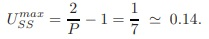
\includegraphics[width=8cm, height=1.5cm]{alg2}
	\caption{ Maximum Server Utilization}
	\centering
\end{figure}

\begin{figure}[h!]
	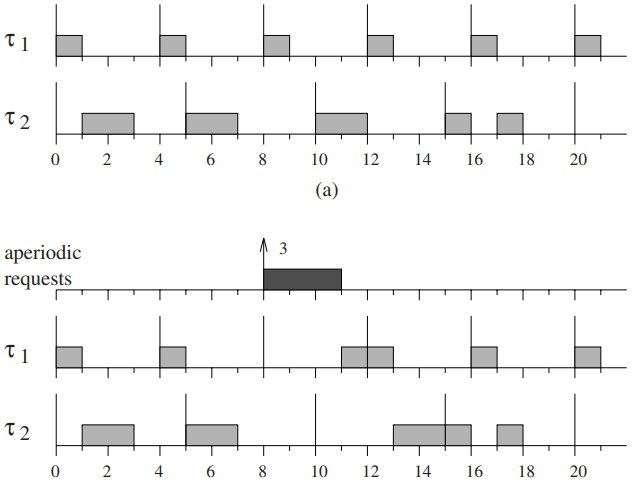
\includegraphics[width=8cm, height=6cm]{behavior}
	\caption{Slack Stealing Behavior}
	\centering
\end{figure}

This means that, even with Cs = 1, the shortest server period that can be set with
this utilization factor is Ts = [Cs/Us] = 7, which is greater than both task periods.
Thus, the execution of the server would be equivalent to a background service, and the
aperiodic request would be completed at time 15.

In order to schedule an aperiodic request Ja(ra, Ca) according to the Slack Stealing
algorithm, we need to determine the earliest time t such that at least Ca units of slack
are available in [ra, t]. The computation of the slack is carried out through the use of
a slack function A(s, t), which returns the maximum amount of computation time that
can be assigned to aperiodic requests in the interval [s, t] without compromising the
schedulability of periodic tasks.
Figure 6 shows the slack function at time s = 0 for the periodic task set considered
in the previous example. For a given s, A(s, t) is a non-decreasing step function
defined over the hyperperiod, with jump points corresponding to the beginning of the
intervals where the slack is available. As s varies, the slack function needs to be
recomputed, and this requires a relatively large amount of calculation, especially for
long hyperperiods. Figure 7 shows how the slack function A(s, t) changes at time
s = 6 for the same periodic task set.
According to the original algorithm,
the slack function at time s = 0 is precomputed and stored in a table. During runtime,
the actual function A(s, t) is then computed by updating A(0, t) based on the periodic execution time, the aperiodic service time, and the idle time. The complexity for
computing the current slack from the table is O(n), where n is the number of periodic
tasks; however, depending on the periods of the tasks, the size of the table can be too
large for practical implementations.
\begin{figure}[h!]
	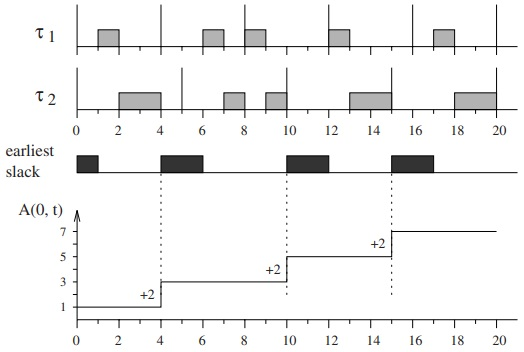
\includegraphics[width=8cm, height=6cm]{behavior2}
	\caption{Slack Stealing Behavior at Time s = 0}
	\centering
\end{figure}
We can also use an alternative to this algorithm, where the available slack is computed whenever an aperiodic requests enters the system. This method is more complex than the
previous static approach, but it requires much less memory and allows handling of
periodic tasks with release jitter or synchronization requirements. 

\begin{figure}[h!]
	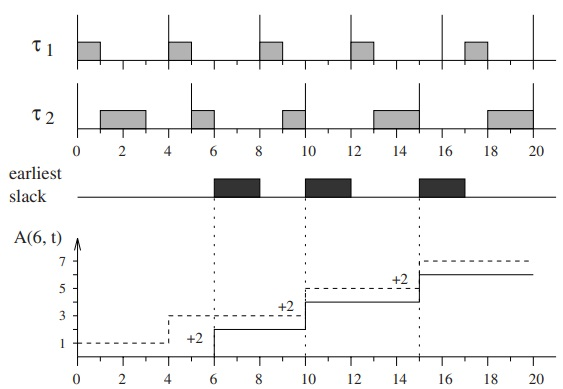
\includegraphics[width=8cm, height=6cm]{behavior3}
	\caption{Slack Stealing Behavior at Time s = 6}
	\centering
\end{figure}

\section {Fast Slack Method}
\subsection{Application}
The Fast Slack method is an alternative use of slack stealing developed by Jose Manuel Urriza, whose example this paper will use, where a set of counters is implemented during runtime in order to reduce the computational cost of the Fast Slack method. 
A set of counters keeps track of the slack which may be stolen at each priority level. 
\begin{figure}[h!]
	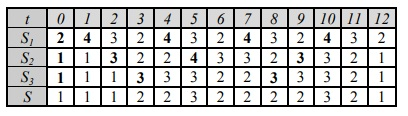
\includegraphics[width=8cm, height=3cm]{table2}
	\caption{Fast Slack Showcase Table}
	\centering
\end{figure}
The slack available to
execute non-critical tasks will be the minimum value of the counters. By analyzing how the slack varies during
runtime, we can state the following rules to manage the counters:

\begin{itemize}
	\item When a lower priority task is executed, higher priority counter should be decremented in an amount equal to the time executed.
	\item When a non-critical task is executed or there exists an idle time, all the counters should be decremented in an amount of time equal to the time consumed.
	\item When a task finishes its execution, the Fast Slack method is calculated to initialize its counter. 
	\item When a task finishes its execution before its Worst Case Execution Time, all lower priority counters
	should be incremented in a time equal to the Worst Case Execution Time minus the time that the task used
	to complete.
\end{itemize}



We can note that if the system is schedulable, then no counter can hold a negative value.
In Figure 8 we can see the counters of the system of the example in the previous section. The bold numbers are basically indicating
that the slack was calculated because the task finished its execution. The last row shows the slack available to execute a
non-critical task. 

\subsection{Results}

In order to compare Stack Stealing to other methods, three different
groups of tasks are used:
\begin{itemize}
	\item Group A: comprised of 10 real-time tasks. The utilization factor of the systems ranges from 0.4 to 0.9 with
	steps of 0.1, and there are 200 real-time systems for each utilization factor. The periods of the tasks follow
	an exponential composition; 4 tasks with periods in the range 25 to 100 units, 3 tasks with periods between
	100 and 1000 units and a further 3 tasks with periods between 1000 and 10000 units.
	\item Group B: comprised of 20 real-time tasks. The utilization factor of the systems ranges from 0.4 to 0.9 with
	steps of 0.1, and there are 200 real-time systems for each utilization factor. The periods of the tasks follow
	an exponential composition; 7 tasks with periods in the range 25 to 100 units, 7 tasks with periods between
	100 and 1000 units and a further 6 tasks with periods between 1000 and 10000 units.
	\item Group C: comprised of 50 real-time tasks. The utilization factor of the systems ranges from 0.5 to 0.9 with
	steps of 0.1, and there are 200 real-time systems for each utilization factor. The periods of the tasks follow
	an exponential composition; 17 tasks with periods in the range 25 to 100 units, 17 tasks with periods
	between 100 and 1000 units and a further 16 tasks with periods between 1000 and 10000 units.
	
\end{itemize}
Each real-time system was generated as follows. First, the periods of the tasks were chosen at random from the
desire range. Deadlines were set equal to the periods. The tasks were then sorted into deadline monotonic priority order. Next, random execution times were assigned, highest priority first. The computation times were constrained
such that the partial task remained feasible according to a sufficient and necessary schedulability test. Finally tasks
sets with an utilization level differing by more than 0.5\% from that required were discarded. We simulated each
real-time system for 15 consecutives releases of the lowest priority tasks after the worst case of load. We counted
the number of iterations that each algorithm needs to get the slack available. The results presented are the averages
over each group. 
Figure 9 shows the average number of iterations for each utilization factor of groups A, B and C that Fast Slack
and the alternative slack-stealing mechanism required to get the slack available. We can note that the number
of iterations that Fast Slack requires is much less for low utilization factors and remains lower for high utilization
factors.
\begin{figure}[h!]
	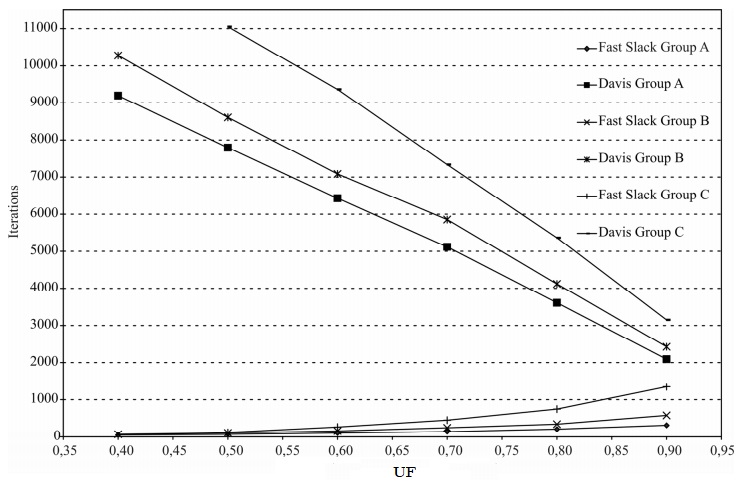
\includegraphics[width=8cm, height=6cm]{graph}
	\caption{Comparison of Fast Slack and Other Methods}
	\centering
\end{figure}
From these results we can conclude that the number of iterations that Fast Slack requires increases as the
utilization factor increases because the inspection interval increases as well and consequently the equation should be
calculated more times.
The number of iterations of the method proposed previously decreases as the utilization factor increases because it
calculates the slack based on the intervals when the system is idle. At low utilization factors the systems is idle most of the time and consequently the mechanism has to be evaluated at each one of these idle intervals. As the
utilization factor increases, the number of idle intervals decreases and then the number of iteration decreases.
The simulations were performed considering integer execution times. When fractional executions times are
considered, then the Davis’s method (as an alternative to the Slack Stealing one) increases the number of iterations whilst the Fast Slack method remains with
the same performance. 

\section{Approximate slack stealing algorithms}
\subsection{Delineation}
Another useful topic to discuss is approximations to the optimal
dynamic algorithm. The objective is to produce slack
stealing algorithms which are efficient enough for runtime usage. First we consider stealing slack from purely
periodic task sets. We indicate how our analysis can be
used in an algorithm which replicates the behavior of an
optimal Slack Stealer. We
then present an approximate algorithm which can be used
to steal slack from both hard deadline periodic and
sporadic tasks. We compare the performance of this
algorithm to the optimal and background processing
methods. Finally, we discuss the overheads of the
approximate algorithm and their justification in terms of
improved soft task response times.
For hard deadline periodic task sets, the slack available
at priority level i only increases when task i completes.
We may therefore replicate the behavior of an optimal Slack
Stealer by using an algorithm (Figure 10) to calculate Smax at each completion of task i.
\begin{figure}[h!]
	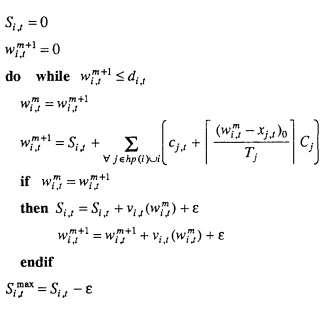
\includegraphics[width=8cm, height=5.5cm]{alg3}
	\caption{Task i Algorithm}
	\centering
\end{figure}
Figure 11 (a and b) are then used to keep track of the
slack available at other times. The overhead of computing
the slack can be reduced by a priori calculation of the
least additional slack, Sadd, which becomes available at
every completion of task i. This enables a less pessimistic
initial value for Sid to be used in Figure 10, thus
reducing computation.
\begin{figure}[h!]
	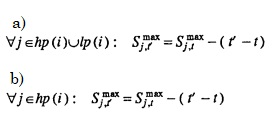
\includegraphics[width=8cm, height=3cm]{alg4}
	\caption{Dynamic Algorithm}
	\centering
\end{figure}
The least additional level i slack is generated when
task i completes as late as possible (i.e. at its deadline) and
the subsequent invocation is subject to the maximum
interference from higher priority tasks. Maximum
interference occurs when all higher priority tasks are
released at the above deadline. This is effectively a
critical instant for task i. Thus is equivalent to
the level i idle time in the interval [O , Ti) where time 0 is
a critical instant. The algorithm in Figure 10 may be used to calculate
the value of Sadd off-line.
We may implement a simple slack stealing algorithm
by incrementing the level i slack available by Sadd at each
completion of task i, whilst again using the equations in Figure 11 (a and b) to keep track of the slack at other times. The
approximate slack stealing algorithm comprises this
simple algorithm augmented by periodically evaluating the exact slack available at all priority levels. Varying the
period at which this is done enables the overhead of the
dynamic slack stealer to be traded off against a decrease in
the responsiveness of soft tasks. A very short period
minimizes the response times of soft tasks at the expense
of a large overhead (c.f. the optimal dynamic algorithm).
Whilst a very long period minimizes the overhead, but
increases the response times. In the next section, we
examine this performance trade-off. 

\subsection{Results}
For evaluation purposes, sets of hard deadline
periodic tasks were used, enabling comparisons to be made between
the approximate algorithm described above and the
optimal Slack Stealer algorithm. The
results are averaged over 10 task sets, each comprising 10
hard deadline periodic tasks. The periods of the hard
deadline tasks were chosen at random in the range 2 to
1000 ticks. Deadlines were randomly chosen, but
constrained to be less than or equal to the period. Finally
computation times were adjusted randomly until the total
processor utilization of the hard deadline task set was
approximately 50\%. Each task set was then subject to a
sufficient and necessary schedulability test. Unschedulable
task sets were discarded.

\begin{figure}[h!]
	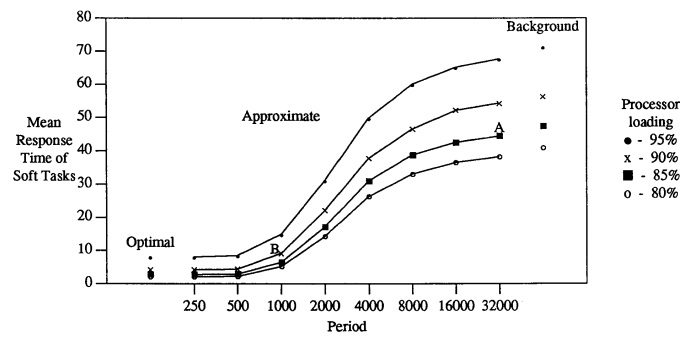
\includegraphics[width=9cm, height=5.5cm]{graph2}
	\caption{Approximate Slack Stealing Result Graph}
	\centering
\end{figure}

The soft task load was simulated by a FIFO queue of
tasks, each requiring 1 tick of processing time. The arrival
times of the soft tasks followed a uniform distribution
over the test duration (lo0000 ticks). The number of soft
tasks was varied to produce a simulated total processor
loading of 80\%, 85\%, 90\% and 95\%. For each utilization
level, we recorded the response time of each soft task
scheduled by background, optimal and approximate slack
stealing algorithms. In the case of the approximate
algorithm, the simulation was repeated using periods of
250,500, 1000,2000,4000,8000, 16000 and 32000 ticks
between calculations of the exact slack available.
For comparison purposes, the mean
response times of soft tasks scheduled by the optimal
algorithm are plotted on the left, whilst corresponding
values for background processing are plotted on the right (Figure 12).
The graph shows that for all "loadings" the mean response
time of soft tasks, scheduled by the approximate
algorithm, was very close to the optimal provided the
period of the approximate algorithm was less than the
mean task period (500 ticks). Increasing the period of the
approximate algorithm resulted in decreased
responsiveness, until with a large period (32000), it was
close to that of background.

\section{Conclusion}
The apparent versatility and, almost paradoxically, the strict nature of its definition, allow for a useful and predictable tool for Real-Time embedded systems. Its performance and its load on any system can be adjusted flexibly, allowing for a greater degree in practicality. It is safe to say that Stack Stealing will stand the test of time in the current generation of computing. 

\section{Statement of Originality}
I hereby declare that this submission is my own work and to the best of my
knowledge it contains no materials previously published or written by another
person, or substantial proportions of material which have been accepted for the
award of any other degree or diploma at HSHL or any other educational
institution, except where due acknowledgment is made in the thesis. Any
contribution made to the research by others, with whom I have worked at
HSHL or elsewhere, is explicitly acknowledged in the thesis. I also declare that
the intellectual content of this research paper is the product of my own work, except to
the extent that assistance from others in the project's design and conception or
in style, presentation and linguistic expression is acknowledged.

\begin{thebibliography}{9}
	\bibitem{eth} 
	C. Buttazzo,
	\textit{Hard real-time computing systems: predictable scheduling algorithms and applications} 
	, 3rd ed. New York: Springer, 2011 \\
	Figures 1,3-7 are from this material.
	
	\bibitem{eth2} 
	Douglas Wilhelm Harder, Jeff Zarnett,
	Vajih Montaghami and Allyson Giannikouris,
	\textit{A practical introduction
		to real-time systems
		for undergraduate engineering}, 2014 \\ Figure 2 is from this material
	\hfill
	
	\bibitem{eth3} 
	Jose Manuel Urriza,
	\textit{A Fast Slack Stealing method for embedded Real-Time Systems}, 2005 \\
	Figures 8 and 9 are from this material
	\hfill
	
	\bibitem{eth4} 
	R.I.Davis, K.W.Tindel1, ABurns ,
	\textit{Scheduling Slack Time in Fixed Priority Pre-emptive Systems}, 1993 \\
	Figures 10-12 are from this material
	\hfill
	
	\bibitem{eth} 
	R. Mall,
	\textit{Real-Time Systems: Theory and Practice}, 2009
	\hfill
	
	Other material used:
	\begin{itemize}
		\item [1] Slack Stealing - Real Time System: Chapter 5 (https://www.youtube.com/watch?v=9VA4eyT5w2M\&ab
		\_channel=SagunRajLage)
		\item [2] What is Slack Stealing in Deadline Driven System? (https://www.youtube.com/watch?v=5U\_pLwPtVY4\&ab
		\_channel=InformationTechnologyHelpDeskOnline)
				
	\end{itemize}
	
\end{thebibliography}

\end{document}
